\documentclass[a4paper,12pt]{article}
\usepackage[utf8]{inputenc}
\usepackage[T1]{fontenc}
\usepackage[italian]{babel}
\usepackage{graphicx}
\usepackage{hyperref}
\usepackage{amsmath}

\title{Relazione -- Settimana 2}
\author{Gruppo di Lavoro}
\date{\today}

\begin{document}

\maketitle

\section*{Introduzione e Obiettivi}
Nel corso della seconda settimana di lavoro, ci siamo concentrati sulla definizione del \textbf{dataset iniziale} necessario all’addestramento di BERT, sull’analisi del flusso di elaborazione e sulla scelta degli strumenti di traduzione per gestire risposte in lingue diverse dall’inglese. In particolare, abbiamo approfondito la \emph{strategia di test} che prevede di utilizzare una versione più leggera di BERT su Google Colab, per poi passare a una variante più potente da eseguire sul cluster del dipartimento.

\section*{Definizione del Dataset}
Dopo una valutazione delle risorse disponibili e in accordo con il professore, abbiamo deciso di creare un \textbf{pool iniziale di 4.000 esempi}, di cui:
\begin{itemize}
    \item \textbf{2.000 esempi di risposte “non jailbreak”}, ritenute valide o in linea con le policy;
    \item \textbf{2.000 esempi di risposte “jailbreaked”}, in cui l’LLM è stato indotto a produrre output non conformi o a violare determinati vincoli.
\end{itemize}

La soglia di 2.000 esempi per parte è stata scelta sia per la disponibilità limitata di risposte jailbreaked, sia per mantenere la fase di \emph{fine-tuning} più gestibile dal punto di vista computazionale. Le nostre ricerche iniziali suggerivano un range compreso tra 2.000 e 5.000 esempi per parte, e la scelta di rimanere su 2.000 è un compromesso tra \emph{qualità} del dataset e \emph{fattibilità} dell’esperimento.

\paragraph{Scrematura del Dataset}
Abbiamo previsto una fase di \emph{scrematura} (prevista per la prossima settimana) non appena il professore ci metterà a disposizione il \emph{dataset iniziale} generato durante i test di \emph{jailbreaking}. Questa scrematura servirà a eliminare dati duplicati, inconsistenti o privi di etichette affidabili, così da garantire la massima coerenza del set di addestramento.

\section*{Strategia di Test su Google Colab}
Uno dei punti centrali emersi questa settimana riguarda la \textbf{necessità di testare il processo di fine-tuning} su un modello più leggero di BERT, da eseguire su \emph{Google Colab}. Questa scelta nasce dall’esigenza di:
\begin{itemize}
    \item Validare rapidamente l’approccio su un dataset di dimensioni ridotte, monitorando metriche come accuratezza, precisione e recall;
    \item Familiarizzare con il \emph{fine-tuning} di BERT in ambiente Colab, identificando eventuali colli di bottiglia (tempo di training, memoria GPU, ecc.);
    \item Evitare sprechi di risorse sul cluster del dipartimento, riservandolo a fasi successive, più impegnative computazionalmente.
\end{itemize}

Una volta completata questa fase di test e \textbf{validata} l’efficacia del dataset (in termini di risultati ottenuti), prevediamo di:
\begin{enumerate}
    \item Eseguire il \emph{fine-tuning} di una \emph{versione più potente di BERT} sul cluster del dipartimento, sfruttando l’hardware più performante;
    \item Salvare il modello addestrato su \emph{Hugging Face}, in modo da poterlo integrare facilmente in diversi ambienti di sviluppo \emph{Python}.
\end{enumerate}

\section*{Introduzione di un Layer di Traduzione}
Rianalizzando lo \emph{schema generale} del sistema, ci siamo resi conto che non si può assumere che le risposte dell’LLM siano esclusivamente in lingua inglese. Per questo motivo, abbiamo deciso di \textbf{introdurre un layer di traduzione} che converta eventuali testi in lingue diverse dall’inglese, in modo da standardizzare l’input prima di inviarlo a BERT.

\paragraph{Librerie Python per la Traduzione}
Abbiamo esplorato diverse \emph{librerie Python} che consentono di effettuare traduzioni in modo \emph{batch} o \emph{on-the-fly}. Alcune di queste librerie si interfacciano direttamente con servizi esterni (ad esempio \emph{Google Translate}), mentre altre si basano su modelli open source. L’idea è di scegliere la soluzione che offra il miglior compromesso tra:
\begin{itemize}
    \item \emph{Qualità della traduzione}: importante per non introdurre distorsioni semantiche nel testo di input;
    \item \emph{Velocità di esecuzione}: necessaria per non rallentare eccessivamente il \emph{pipeline} di valutazione;
    \item \emph{Costi e limiti di API}: in caso di utilizzo di servizi esterni.
\end{itemize}

\section*{Schema Aggiornato della Soluzione}
Nella Figura~\ref{fig:flusso2} riportiamo il \textbf{nuovo schema} del sistema, in cui si evidenzia il \emph{layer di traduzione} prima dell’elaborazione da parte di BERT.

\begin{figure}[h!]
    \centering
    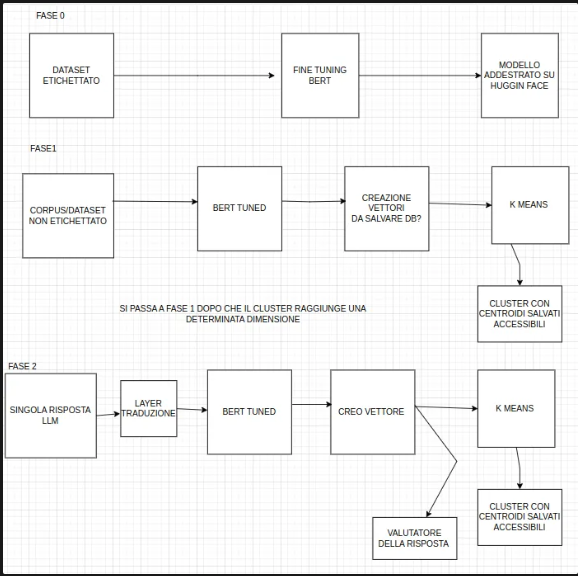
\includegraphics[width=0.7\textwidth]{image.png} % Sostituire con il nome effettivo del file immagine
    \caption{Schema aggiornato della soluzione, con l’aggiunta del layer di traduzione.}
    \label{fig:flusso2}
\end{figure}

\section*{Analisi dei Dati per il Clustering}
Oltre all’addestramento di BERT, ci siamo posti il problema di quante risposte saranno necessarie per la fase di \emph{clustering} tramite \emph{k-means}. In particolare:
\begin{itemize}
    \item \textbf{Dataset per il clustering}: potremmo utilizzare lo stesso \emph{dataset} di addestramento di BERT, integrato con ulteriori esempi, per ottenere una varietà di vettori sufficientemente ampia da garantire la robustezza dei centroidi.
    \item \textbf{Aggiornamento dinamico o statico}: non abbiamo ancora stabilito se, a regime, i cluster dovranno aggiornarsi con l’arrivo di nuove risposte. Questa scelta dipenderà dalla \emph{qualità} e \emph{stabilità} delle previsioni di BERT e dal \emph{tasso} con cui si generano nuovi dati.
\end{itemize}

\section*{Ricerca Implementativa e Documentazione}
Abbiamo proseguito il lavoro di ricerca sulle \textbf{soluzioni implementative in Python}, analizzando vari \emph{video} e \emph{materiali} relativi al \emph{fine-tuning} di BERT. Come di consueto, tutto il materiale raccolto (librerie, tutorial, esempi di codice) sarà inserito o collegato su \emph{Notion}, così da garantire la condivisione del sapere e la possibilità di riprodurre i passaggi di configurazione in futuro.

\section*{Conclusioni e Prospettive}
In sintesi, la seconda settimana di lavoro si è concentrata su:
\begin{itemize}
    \item \textbf{Definire} la dimensione e la composizione del dataset iniziale (4.000 esempi bilanciati tra risposte jailbreaked e non jailbreaked);
    \item \textbf{Pianificare} la fase di test su \emph{Google Colab} con una versione leggera di BERT, per poi passare a un modello più potente sul cluster del dipartimento;
    \item \textbf{Inserire} un layer di traduzione nel \emph{pipeline}, al fine di gestire risposte multilingue e garantire la coerenza dell’input a BERT;
    \item \textbf{Analizzare} le esigenze in termini di dati per la creazione dei cluster \emph{k-means}, valutando la possibilità di un aggiornamento dinamico.
\end{itemize}

Nella prossima settimana, contiamo di:
\begin{itemize}
    \item Ricevere e \emph{scremare} il dataset dal professore, eliminando dati non validi o ridondanti;
    \item Avviare i primi esperimenti di \emph{fine-tuning} su BERT Base in ambiente Colab;
    \item Proseguire lo studio dei \emph{modelli di traduzione} e definire la pipeline definitiva di elaborazione del testo.
\end{itemize}

\end{document}
